
\noindent 
This unit covers the following ideas. In preparation for the quiz and exam, make sure you have a lesson plan containing examples that explain and illustrate the following concepts.  
\begin{enumerate}

\item Be able to convert between rectangular and polar coordinates in 2D. Convert between rectangular and cylindrical or spherical in 3D. \valpo{Topical Objective \# 15}
\item Graph polar functions in the plane. Find intersections of polar equations, and illustrate that not every intersection can be obtained algebraically (you may have to graph the curves).
\item Find derivatives and tangent lines in polar coordinates.
\item Find area and arc length using polar equations.

\end{enumerate}
You'll have a chance to teach your examples to your peers prior to the exam.

\section{Polar Coordinates}
Up to now, we most often give the location of a point (or coordiantes of a vector) by stating the $(x,y)$ coordinates.  These are called the Cartesian (or rectangular) coordinates.  Some problems are much easier to work with if we know how far a point is from the origin, together with the angle between the $x$-axis and a ray from the origin to the point.

\begin{problem}
\marginpar{
	\thomasee{See 11.3:5-10.}
	}%
There are two parts to this problem.
\begin{enumerate}
\item Consider the point $P$ with Cartesian (rectangular) coordinates $(2,1)$.  Find the distance $r$ from $P$ to the origin. Consider the ray $\vec {OP}$ from the origin through $P$. Find an angle between $\vec{OP}$ and the $x$-axis. 

\item Suppose that a point $Q=(a,b)$ is 6 units from the origin, and the angle the ray $\vec {OP}$ makes with the $x$-axis is $\pi/4$ radians.  Find the Cartesian (rectangular) coordinates $(a,b)$ of $Q$.
\end{enumerate}

 
\end{problem}

\begin{definition}
Let $Q$ be be a point in the plane with Cartesian coordinates $(x,y)$.  Let $O=(0,0)$ be the origin. We define the polar coordinates of $Q$ to be the ordered pair $(r,\theta)$ where $r$ is the displacement from the origin to $Q$, and $\theta$ is an angle of rotation (counter-clockwise) from the $x$-axis to the ray $\vec {OP}$.
\end{definition}

\begin{problem}  
\marginpar{
	\thomasee{See 11.3:5-10.}
	}%
The following points are given using their polar coordinates.  Plot the points in the Cartesian plane, and give the Cartesian (rectangular) coordinates of each point. The points are
$$
(1,\pi), 
\ds \left( 3,\frac{5\pi}{4}\right),
\ds \left( -3,\frac{\pi}{4}\right),\text{ and }
\ds \left( -2,-\frac{\pi}{6}\right).$$
\end{problem}

The next problem provides general formulas for converting between the Cartesian (rectangular) and polar coordinate systems.

\begin{problem}\label{polar coordinate equations}  
\marginpar{
	\thomasee{See page 647.}
	}%
Suppose that $Q$ is a point in the plane with Cartesian coordinates $(x,y)$ and polar coordinates $(r,\theta)$.  (1) Write formulas for $x$ and $y$ in terms of $r$ and $\theta$.  
Then (2) write a formula to find the distance $r$ from $Q$ to the origin (in terms of $x$ and $y$) as well as (3) a formula to find the angle $\theta$ between the $x$-axis and a line connecting $Q$ to the origin. [Hint: A picture of a triangle will help here.]
\end{problem}
 
In problem \ref{polar coordinate equations}, you should have obtained the equations 
$$x=r\cos\theta, \quad y=r\sin\theta.$$
We can write this in vector notation as $\begin{pmatrix}x\\y\end{pmatrix}=\begin{pmatrix}r\cos\theta\\ r\sin\theta\end{pmatrix}$.
This is a vector equation in which you input polar coordinates $(r,\theta)$ and get out Cartesian coordinates $(x,y)$.  
So you input one thing to get out one thing, which means that we have a function.  
We could write $\vec T(r,\theta) = (r\cos\theta,r\sin\theta)$, where we've used the letter $T$ as the name of the function because it is a transformation between coordinate systems. 
To emphasize that the domain and range are both two dimensional systems, we could also write $T:\mathbb{R}^2\to\mathbb{R}^2$. In the next chapter, we'll spend more time with this notation. The following problem will show you how to graph a coordinate transformation.  When you're done, you should essentially have polar graph paper.

\begin{problem} \label{polar coordinate transformation graph}\marginpar{For this problem, you are just drawing many parametric curves.  This is what we did in the previous chapter.}
Consider the coordinate transformation $$\vec T(r,\theta) = (r\cos\theta,r\sin\theta).$$ 
\begin{enumerate}
\item Let $r=3$ and then graph $\vec T(3,\theta)=(3\cos\theta,3\sin\theta)$ for $\theta\in[0,2\pi]$.
\item Let $\theta=\frac{\pi}{4}$ and then, on the same axes as above, add the graph of 
$\vec T\left(r,\frac{\pi}{4}\right)=\left(r\frac{\sqrt 2}{2},r \frac{\sqrt 2}{2}\right)$ for $r\in[0,5]$.
\item To the same axes as above, add the graphs of 
$\vec T(1,\theta), \vec T(2,\theta), \vec T(4,\theta)$  for $\theta\in[0,2\pi]$ and 
$\vec T(r,0), \vec T(r,\pi/2), \vec T(r,3\pi/4), \vec T(r,\pi)$ for $r\in[0,5]$. 
\end{enumerate}
\end{problem}


\begin{problem} 
In the plane, graph the curve $y=\sin x$ for $x\in[0,2\pi]$ (make an $x,y$ table) and then graph the curve $r=\sin\theta$ for $\theta\in[0,2\pi]$ (an $r,\theta$ table).  The graph should look very different.  If one looks like a circle, you're on the right track.  
\end{problem}

\begin{problem}
\marginpar{
	\thomasee{See 11.3: 53-66.}
	}%
Each of the following equations is written in the Cartesian (rectangular) coordinate system.  Convert each to an equation in polar coordinates, and then solve for $r$ so that the equation is in the form $r=f(\theta)$.
\begin{enumerate}
\item $x^2+y^2=7$
\item $2x+3y=5$
\item $x^2=y$
\end{enumerate}
\end{problem}

\begin{problem} 
\marginpar{
	\thomasee{See 11.3: 27-52. I strongly suggest that you do many of these as practice.}
	}%
Each of the following equations is written in the polar coordinate system.  Convert each to an equation in the Cartesian coordinates.
\begin{enumerate}
\item $r=9\cos\theta$
\item $\ds r=\frac{4}{2\cos\theta+3\sin\theta}$
\item $\theta = 3\pi/4$
\end{enumerate}
\end{problem}

\subsection{Graphing and Intersections}
To construct a graph of a polar curve, just create an $r,\theta$ table. Choose values for $\theta$ that will make it easy to compute any trig functions involved. Then connect the points in a smooth manner, making sure that your radius grows or shrinks appropriately as your angle increases.  

\begin{problem} 
\marginpar{
	\thomasee{See 11.4: 1-20.}
	}%
Graph the polar curve $r=2+2\cos\theta$.
\end{problem}

\begin{problem}
Graph the polar curve $r=2\sin 3\theta$.
\end{problem}

\begin{problem}
Graph the polar curve $r=3\cos 2\theta$.
\end{problem}


\begin{problem}
Find the points of intersection of $r=3-3\cos\theta$ and $r=3\cos\theta$. (If you don't graph the curves, you'll probably miss a few points of intersection.)
\end{problem}

\begin{problem}
Find the points of intersection of $r=2\cos 2\theta $ and $r=\sqrt 3$. (If you don't graph the curves, you'll probably miss a few points of intersection.)
\end{problem}


\subsection{Calculus with Polar Coordinates}

Recall that for parametric curves $\vec r(t) = (x(t),y(t))$, to find the slope of the curve we just compute $$\frac{dy}{dx}=\frac{dy/dt}{dx/dt}.$$ A polar curve of the form $r=f(\theta)$ can be thought of as just the parametric curve $(x,y) = (f(\theta)\cos\theta,f(\theta)\sin\theta)$. So you can find the slope by computing
$$\frac{dy}{dx}=\frac{dy/d\theta}{dx/d\theta}.$$

\begin{problem}
\marginpar{
	\thomasee{See 11.2: 1-14.}
	}%
Consider the polar curve $r=1+2\cos \theta$. (It wouldn't hurt to provide a quick sketch of the curve.)
\begin{enumerate}
\item Compute both $dx/d\theta$ and $dy/d\theta$.
\item Find the slope $dy/dx$ of the curve at $\theta=\pi/2$.
\item Give both a vector equation of the tangent line, and a Cartesian equation of the tangent line at $\theta=\pi/2$.
\end{enumerate}
\end{problem}

We showed in the curves section that you can find arc length for parametric curves using the formula 
$$s=\int_a^b\sqrt{\left(\frac{dx}{dt}\right)^2+\left(\frac{dy}{dt}\right)^2}.$$ If we replace $t$ with $\theta$, this becomes a formula for arc length in polar coordinates.  However, the formula can be simplified.

\begin{problem}
\marginpar{
	\thomasee{See 11.5: 29.}
	}%
Recall that $x=r\cos\theta$ and $y=r\sin\theta$. Suppose that $r=f(\theta)$ for $\theta\in[\alpha,\beta]$ is a continuous function, and that $f'$ is continuous.  
Show that the arc length formula can be simplified to 
$$
s=\int_{\alpha}^{\beta}\sqrt{\left(\frac{dx}{d\theta}\right)^2+\left(\frac{dy}{d\theta}\right)^2} 
= \int_{\alpha}^{\beta}\sqrt{r^2+\left(\frac{dr}{d\theta}\right)^2} .$$
[Hint: the product rule and Pythagorean identity will help.]
\end{problem}

\begin{problem} 
\marginpar{
	\thomasee{See 11.5: 21-28.}
	}%
Set up (do not evaluate) an integral formula to compute the length of 
\begin{enumerate}
\item the rose $r=2\cos 3\theta$, and
\item the rose $r=3\sin 2\theta$.
\end{enumerate}
\end{problem}


\begin{problem}
\marginpar{
	\thomasee{See page 653.}
	}%
In this problem, you will develop a formula for finding area inside a polar curve.
\begin{enumerate}
\item 
Consider a circle of radius $r$. The area inside the circle is $\pi r^2$. This is the area inside when you traverse around the circle for a full $2\pi$ radians.  Fill in the following table by finding the pattern that connects angle traversed to area inside.
\begin{center}
\begin{tabular}{c|c}
Angle traversed& Area inside\\ \hline
$2\pi$ & $A=\pi r^2$\\
$\pi$ & \\
$\pi/2$ & \\
$\pi/4$ & \\
$d\theta$ & $dA=\quad\quad$
\end{tabular}
\end{center}
\item Explain why the area inside a polar curve $r=f(\theta)$ for $\alpha\leq \theta\leq \beta$ is $$A = \int dA = \int_\alpha^\beta \frac{1}{2}r^2d\theta.$$
What must be true about the curve $r=f(\theta)$ for this formula to be valid?
\end{enumerate}
\end{problem}

\begin{problem} 
\marginpar{
	\thomasee{See 11.5: 1-20.}
	}%
Find the area inside of the polar curve $r=\sin\theta$. [Hint: Construct a graph to determine the appropriate bounds for the integral. When you integrate, you'll need to use the half angle identity.] 
\end{problem}


\begin{problem}
Set up (do not evaluate) an integral to compute the area 
\begin{enumerate}
\item inside the cardioid $r=2+2\sin\theta$, and 
\item inside the circle $r=3\cos\theta$.
\end{enumerate}
\end{problem}

\begin{problem}
Set up (do not evaluate) an integral formula to compute the area that lies inside both $r=2-2\cos\theta$ and $r=\cos\theta$. Sketch both curves. 
\end{problem}


\section{Other Coordinate Systems}
In this chapter, we've introduced just one of many different coordinate systems that people have used over the centuries. Sometimes a problem can't be solved until the correct coordinate system is chosen. Problem \ref{polar coordinate transformation graph} showed you how to graph the coordinate transformation given by polar coordinates.  The following problem shows you how to graph in a different coordinate system.

\begin{problem}
Consider the coordinate transformation $T(a,\omega)=(a\cos\omega,a^2\sin \omega)$.
\begin{enumerate}
\item\marginpar{See
    \href{http://aleph.sagemath.org/?z=eJwti7sKwCAMAHe_IjglkqHY2b9wbgkiJVAfqP9PB7vdHVxE4VbyIxRQXGoTtzHI5d3U-juZPrQusBElnAQ6LcNm02VIyWtouvvbFu7MsFeGg8G7rkQfMv4giA}{Sage}.
  Click on the link to see how to check your answer in Sage.}%
 Let $a=3$ and then graph the curve $\vec T(3,\omega)=(3\cos\omega,9\sin\omega)$ for $\omega\in[0,2\pi]$.
\item\marginpar{See
    \href{http://aleph.sagemath.org/?z=eJxlzEEKg0AMBdC9pwiukmmgRd3OLVxbgkgJqBNm5v5UTGmF7vKT9zOicNqWl1BECXMq6IlBpi4U3T-ZGsu6V2hHlNgTaGkZfP5dThpN78MXXFaNSZZtqVnnp62potcZHDE8GLpgSgQ3-LeXT0fF-UD0BkVHOdw}{Sage}. Notice that you can add the two plots together to superimpose them on each other.}%
 Let $\theta=\frac{\pi}{4}$ and then, on the same axes as above, add the graph of 
$\vec T\left(a,\frac{\pi}{4}\right)=\left(a\frac{\sqrt 2}{2},a^2 \frac{\sqrt 2}{2}\right)$ for $a\in[0,4]$.
\item\marginpar{Use Sage to check your answer.}To the same axes as above, add the graphs of 
$\vec T(1,\omega), \vec T(2,\omega), \vec T(4,\omega)$  for $\omega\in[0,2\pi]$ and 
$\vec T(a,0), \vec T(a,\pi/2), \vec T(a,-\pi/6)$ for $a\in[0,4]$. 
\end{enumerate}
[Hint: when you're done, you should have a bunch of parabolas and ellipses.]
\end{problem}

\newpage
In 3 dimensions, the most common coordinate systems are cylindrical and spherical.  The equations for these coordinate systems are in the table below. 
\bmw{
\begin{center}
\begin{tabular}{cc}
Cylindrical Coordinates & Spherical Coordinates\\
\hline
$\begin{array}{l}
x=r\cos\theta\\
y=r\sin\theta\\
z=z
\end{array}$
&
$\begin{array}{l}
x=\rho\sin\phi\cos\theta\\
y=\rho\sin\phi\sin\theta\\
z=\rho\cos\phi
\end{array}$
\end{tabular}
\end{center}
}

\valpo{
\begin{center}
\begin{tabular}{ccc}
Cylindrical Coordinates & Spherical Coordinates & Sphericial (Physics/Engineering)\\
\hline
$\begin{array}{l}
x=r\cos\theta\\
y=r\sin\theta\\
z=z
\end{array}$
&
$\begin{array}{l}
x=\rho\sin\phi\cos\theta\\
y=\rho\sin\phi\sin\theta\\
z=\rho\cos\phi
\end{array}$
&
$\begin{array}{l}
x=r\sin\theta\cos\phi\\
y=r\sin\theta\cos\phi\\
z=r\cos\theta
\end{array}$ \\
\ 
& \includegraphics{157px-3D_Spherical.eps} \footnote{\valpo{\small{`3D Spherical 2' by Dmcq - Own work. Licensed under Creative Commons Attribution-Share Alike 3.0 via Wikimedia Commons - \href{http://commons.wikimedia.org/wiki/File:3D_Spherical_2.svg\#mediaviewer/File:3D_Spherical_2.svg}{Wikipedia File} } } }

& \includegraphics{157px-3D_Spherical_2.eps} \footnote{\valpo{\small{`3D Spherical' by Andeggs - Own work. Licensed under Public domain via Wikimedia Commons - \href{http://commons.wikimedia.org/wiki/File:3D_Spherical.svg\#mediaviewer/File:3D_Spherical.svg}{Wikipedia File} }}}
\end{tabular}
\end{center}

}

\begin{problem} 
\marginpar{
	\thomasee{See page 893.} 
	\stewarts{See pages 827-833} 
	\larsonfive{See Larson 11.7.}
	}%
Let $P=(x,y,z)$ be a point in space. This point lies on a cylinder of radius $r$, where the cylinder has the $z$ axis as its axis of symmetry.  The height of the point is $z$ units up from the $xy$ plane. The point casts a shadow in the $xy$ plane at $Q=(x,y,0)$.  The angle between the ray $\vec{OQ}$ and the $x$-axis is $\theta$. Construct a graph in 3D of this information, and use it to develop the equations for cylindrical coordinates given above.
\end{problem}

\begin{problem}\label{derive spherical coordinates} Let 
\marginpar{
	\thomasee{See page 897.}
	\larsonfive{See Larson 11.7.}
	}% 
  $P=(x,y,z)$ be a point in space. This point lies on a sphere of
  radius $\rho$ (``rho''), where the sphere's center is at the origin
  $O=(0,0,0)$. The point casts a shadow in the $xy$ plane at
  $Q=(x,y,0)$.  The angle between the ray $\vec{OQ}$ and the $x$-axis
  is $\theta$, and is called the azimuth angle. The angle between
  the ray $\vec{OP}$ and the $z$ axis is $\phi$ (``phi''), and is
  called the inclination angle, polar angle, or zenith angle.  Construct
  a graph in 3D of this information, and use it to develop the
  equations for spherical coordinates given above.
\end{problem}

\marginpar{See the
  \href{http://en.wikipedia.org/wiki/Spherical_coordinate_system}{Wikipedia}
  or
  \href{http://mathworld.wolfram.com/SphericalCoordinates.html}{MathWorld}
  for a discussion of conventions in different disciplines.}%
	
There is some disagreement between different fields about the notation
for spherical coordinates.  In some fields (like physics), $\phi$
represents the azimuth angle and $\theta$ represents the inclination
angle.  In some fields, like geography, instead of the inclination angle, the
\emph{elevation} angle is given---the angle from the $xy$-plane (lines
of lattitude are from the elevation angle).
Additionally, sometimes the coordinates are written in a different
order.  You should always check the notation for spherical coordinates
before communicating using them.


\clearpage

%%% Local Variables: 
%%% mode: latex
%%% TeX-master: "215-problems"
%%% End: 
